% =====================================================================
%  Introduction to Deep Learning — Class 29
%  Topic (course plan): Recurrent Neural Network
%  Subtopic (course plan): RNN for NLP tasks
%  Sources (course plan): Jurafsky & Martin Ch. 13 (Ch. 14 in the
%    August 2026 draft), Goodfellow Ch. 10
%
%  Classes 27 and 28 built the encoder-decoder and opened the cell.
%  This class puts the cell to work on the four output structures of
%  Jurafsky Fig. 14.15 — language modelling, sequence labelling,
%  sequence classification, and (recalled) the encoder-decoder — and
%  on the two ways of combining RNNs as modules: stacking and
%  bidirectionality.  It closes with Goodfellow's reading of the RNN as
%  a graphical model, and the recursive net as the tree-shaped cousin.
%
%  Every measured figure is produced by src/ on the tape of Class 27:
%  a character-level LSTM language model trained on a short
%  public-domain story, two taggers on a small grammar, three
%  classifiers on a signal task.  One result (the gradient paths of
%  the three read-outs) is stated in neither textbook; the C variant
%  is this deck with it removed.  See _shared/PLAN_Classes26_27_28_29.md.
%
%  Compile:  xelatex main.tex   (run twice)
% =====================================================================
\documentclass[aspectratio=169, 11pt]{beamer}

\usetheme{metropoliscustom}

\usepackage{graphicx}
\DeclareGraphicsExtensions{.pdf,.png,.jpg}
\graphicspath{{figs/}{Class29_RNN_NLP_Tasks/B_Recreated_Figures/figs/}}
\usepackage{amsmath, amssymb}
\usepackage{bm}
\usepackage{tikz}
\usetikzlibrary{arrows.meta, positioning, calc, decorations.pathreplacing,
                shapes.geometric, fit, backgrounds}
\tcbuselibrary{skins}

\definecolor{shc}{HTML}{341651}
\definecolor{tealc}{HTML}{1C7293}
\definecolor{dpc}{HTML}{800000}
\definecolor{accc}{HTML}{B8860B}

% ---- theorem environments -------------------------------------------
\setbeamertemplate{theorems}[numbered]
\usepackage{remreset}
\makeatletter\@removefromreset{theorem}{section}\makeatother
\renewcommand{\thetheorem}{\arabic{theorem}}
\newtheorem{lemmax}[theorem]{Lemma}
\newtheorem{propx}[theorem]{Proposition}
\newtheorem{corx}[theorem]{Corollary}
\newtheorem{defx}[theorem]{Definition}
\newtheorem{thmx}[theorem]{Theorem}

\newcommand{\bridge}[1]{%
  {\scriptsize\itshape\color{mcMuted} #1\par}\vspace{0.35em}}

\newcommand{\srcline}[1]{%
  \par\vspace{0.25em}%
  {\scriptsize\color{mcMuted}\hfill #1\par}}

\newcommand{\figsource}[1]{{\scriptsize\color{mcMuted} #1}}
\newcommand{\figcap}[2][0.90]{%
  \begin{center}\begin{minipage}{#1\textwidth}\centering
    {\scriptsize\color{mcMuted} #2}
  \end{minipage}\end{center}}

% =====================================================================
\title{Recurrent Neural Networks}
\subtitle{RNNs for NLP Tasks}
\author{Introduction to Deep Learning \ \textperiodcentered\ Class 29}
\institute{}
\date{}

\footleft{Introduction to Deep Learning}
\footright{RNNs for NLP Tasks}
\titlelogos{}

\begin{document}

\maketitle

\begin{frame}{Outline}
  \tableofcontents
\end{frame}

% =====================================================================
\section{The Recurrent Language Model}
% =====================================================================

\begin{frame}{The cell, put to work}
  \vspace{0.05em}
  \begin{itemize}\itemsep0.3em
    \item Class 27 built the encoder--decoder on a cell $g$; Class 28
          opened it. Today the cell is fixed and the question is
          \alert{what to connect to it}
    \item Four output structures: a token at every step
          (\alert{language modelling}), a label at every step
          (\alert{sequence labelling}), one label for the whole sequence
          (\alert{classification}), a new sequence (the
          \alert{encoder--decoder}, Class 27)
    \item Two ways to combine cells: \alert{stack} them, and run one
          \alert{in each direction}
    \item Closing: the RNN as a probabilistic model, and its tree-shaped cousin
  \end{itemize}
  \srcline{Jurafsky \& Martin (2026), \S14.2--14.4, \S14.6; Goodfellow et al.\ (2016), \S10.2.3, \S10.5--10.6.}
\end{frame}

\begin{frame}{Notation for today}
  \vspace{-0.3em}
  {\footnotesize
  \renewcommand{\arraystretch}{1.22}
  \begin{tabular}{@{}l@{\hspace{1.4em}}l@{}}
    $\mathbf{x}_t \in \{0,1\}^{|V|}$ & one-hot token, index $w_t$; $\mathbf{e}_t = \mathbf{E}\mathbf{x}_t$ its embedding, $\mathbf{E} \in \mathbb{R}^{d \times |V|}$\\
    $d$ & the model dimension, shared by embeddings and states\\
    $\mathbf{h}_t = g(\mathbf{U}\mathbf{h}_{t-1} + \mathbf{W}\mathbf{e}_t)$ & the cell of Classes 27--28 (simple, or an LSTM with $\mathbf{c}_t$ inside)\\
    $\hat{\mathbf{y}}_t = \mathrm{softmax}(\mathbf{V}\mathbf{h}_t)$ & output distribution, $\mathbf{V} \in \mathbb{R}^{|V| \times d}$; $\hat{y}_t[k]$ its $k$-th entry\\
    $\mathbf{h}^{f}_t,\ \mathbf{h}^{b}_t$, $[\,\cdot\,;\,\cdot\,]$ & forward and backward states; concatenation\\
    $L_{\mathrm{CE}}$, $\mathrm{PPL}$ & cross-entropy loss; perplexity\\
    $y^{(t)}, h^{(t)}, \tau$ & Goodfellow's superscripts and length, in the graphical-model slides only\\
  \end{tabular}}
  \vspace{0.3em}

  \begin{alertblock}{Two conventions, one line}
    \small Jurafsky: $\mathbf{W}$ input, $\mathbf{U}$ recurrence,
    $\mathbf{V}$ output, time as a subscript. Goodfellow swaps
    $\mathbf{U}$ and $\mathbf{W}$ and writes $y^{(t)}$. This deck keeps
    Jurafsky's letters, as Classes 27--28 did.
  \end{alertblock}
  \srcline{Jurafsky \& Martin (2026), \S14.2.1; Goodfellow et al.\ (2016), \S10.2.}
\end{frame}

\begin{frame}{The recurrent language model, recalled}
  \vspace{-0.45em}
  \begin{defx}[RNN language model]\label{th:lm}
    \small
    At each step $t$,
    \[
      \mathbf{e}_t = \mathbf{E}\mathbf{x}_t, \qquad
      \mathbf{h}_t = g(\mathbf{U}\mathbf{h}_{t-1} + \mathbf{W}\mathbf{e}_t), \qquad
      \hat{\mathbf{y}}_t = \mathrm{softmax}(\mathbf{V}\mathbf{h}_t),
    \]
    and $P(w_{t+1} = k \mid w_{1:t}) = \hat{y}_t[k]$. The probability of a
    sequence is the product of its next-token probabilities,
    $P(w_{1:n}) = \prod_{i=1}^{n} \hat{y}_i[w_i]$.
  \end{defx}
  \vspace{-0.1em}
  {\footnotesize
  \begin{itemize}\itemsep0.16em
    \item Against the $n$-gram model, the context is not $n-1$ tokens
          but \alert{everything so far}, through $\mathbf{h}_{t-1}$; against
          the feedforward model, not a fixed window
    \item Shapes: $\mathbf{E}$ is $d \times |V|$, $\mathbf{U}, \mathbf{W}$ are
          $d \times d$, $\mathbf{V}$ is $|V| \times d$: the vocabulary enters
          only at the two ends
  \end{itemize}}
  \srcline{Jurafsky \& Martin (2026), Eqs.~14.4--14.9, Fig.~14.5; Mikolov et al.\ (2010).}
\end{frame}

\begin{frame}{Training by self-supervision}
  \vspace{-0.4em}
  \begin{center}
    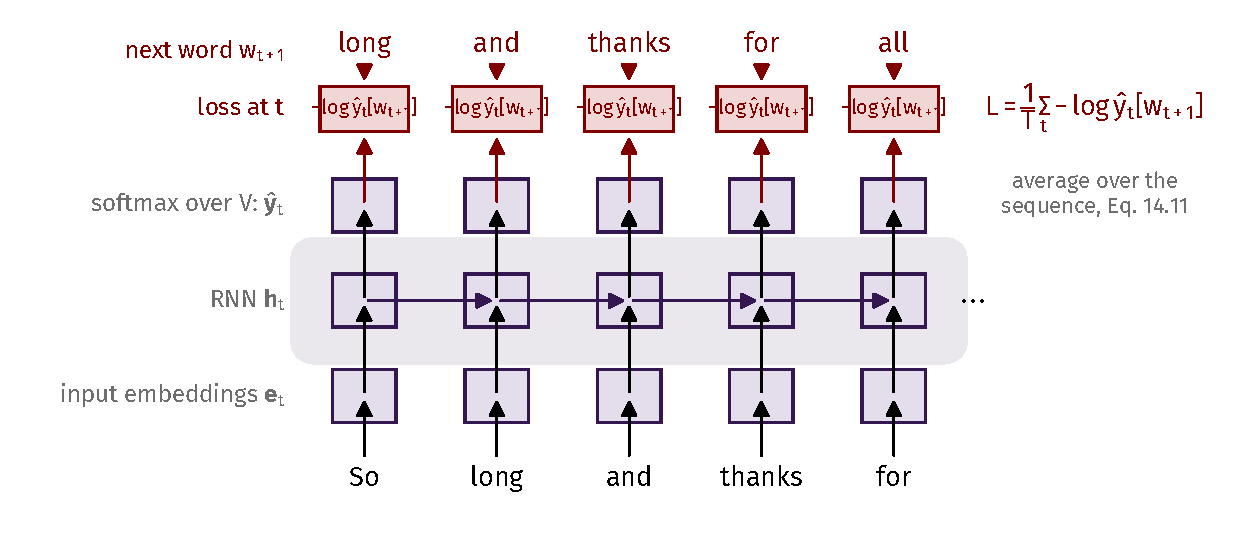
\includegraphics[width=0.80\linewidth]{rnn_lm_training}
  \end{center}
  \vspace{-0.6em}
  {\tiny\color{mcMuted}
  At every position the model reads the true word, predicts the next,
  and pays the cross-entropy of the true next word,
  $L_{\mathrm{CE}}(\hat{\mathbf{y}}_t, \mathbf{y}_t) = -\sum_{w} y_t[w]\log \hat{y}_t[w] = -\log \hat{y}_t[w_{t+1}]$
  for a one-hot target; the loss is the average over the sequence. No
  labels are added: the text is its own supervision. Teacher forcing:
  the input at $t+1$ is the true $w_{t+1}$, not the prediction.
  \hfill Layout of Jurafsky \& Martin (2026), Fig.~14.6.\par}
  \srcline{Jurafsky \& Martin (2026), \S14.2.2, Eqs.~14.10--14.11.}
\end{frame}

\begin{frame}{The training loss is the log of the perplexity}
  \vspace{-0.45em}
  \begin{propx}[Perplexity and cross-entropy]\label{th:ppl}
    \small
    For a text $W = w_1 \ldots w_N$, the perplexity
    $\mathrm{PPL}(W) = P(w_1 \ldots w_N)^{-1/N}$ equals
    $\exp$ of the mean per-token cross-entropy:
    \[
      \mathrm{PPL}(W) = \exp\Big( \frac{1}{N}\sum_{t=1}^{N} -\log P(w_t \mid w_{<t}) \Big).
    \]
  \end{propx}
  \vspace{-0.15em}
  {\footnotesize
  \begin{itemize}\itemsep0.12em
    \item \focus{1}{Proof. By the chain rule
          $P(w_{1:N}) = \prod_t P(w_t \mid w_{<t})$, so
          $-\tfrac{1}{N}\log P(w_{1:N}) = \tfrac{1}{N}\sum_t -\log P(w_t \mid w_{<t})$;
          exponentiate. \hfill $\square$}
    \item \focus{2}{Reading: the \alert{effective number of choices} per
          token --- $|V|$ for a uniform model, $1$ for a perfect one;
          per-token, so texts of different lengths compare. In bits,
          $\mathrm{PPL} = 2^{H(W)}$.}
  \end{itemize}}
  \vspace{-0.3em}
  \srcline{Jurafsky \& Martin (2026), Eqs.~3.14--3.15, 3.42, 7.58.}
\end{frame}

\begin{frame}{A language model, trained}
  \begin{center}
    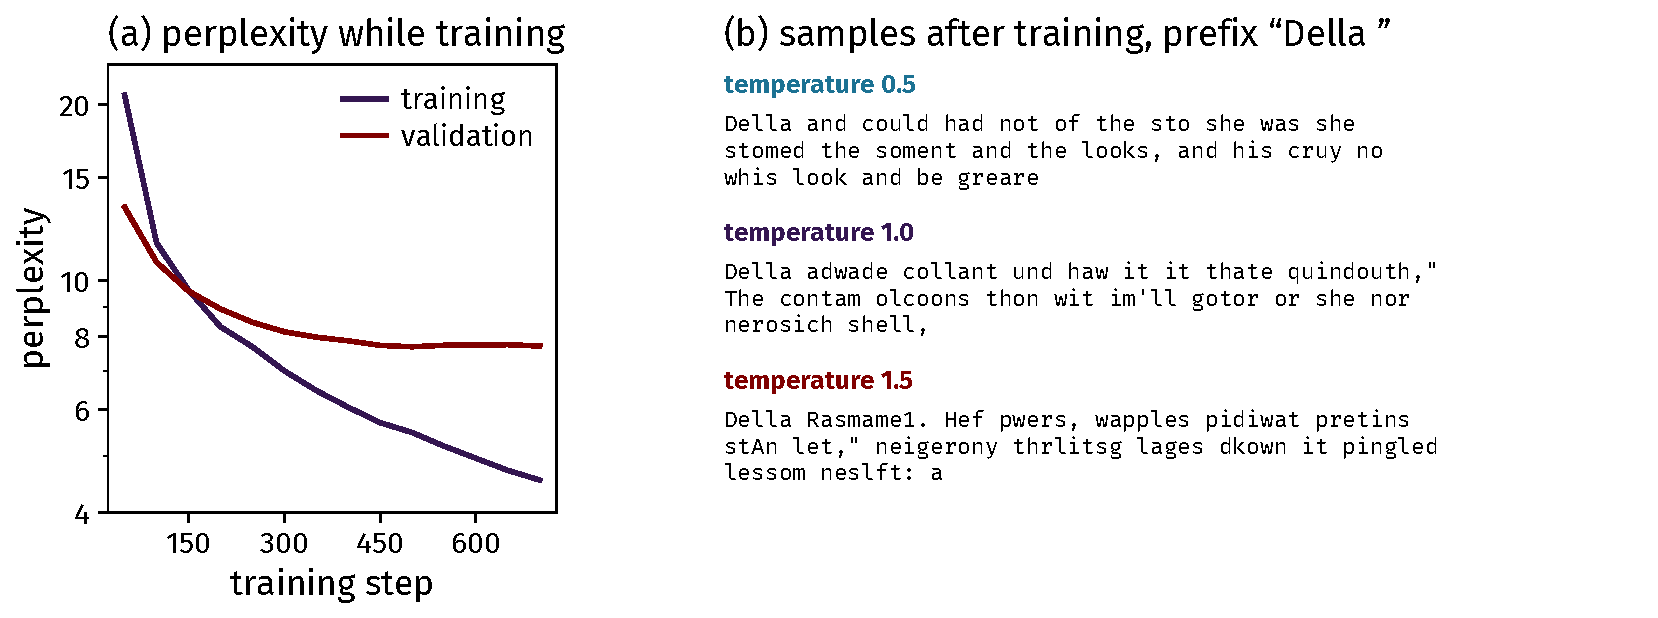
\includegraphics[width=0.90\linewidth]{char_lm}
  \end{center}
  \vspace{-0.6em}
  {\tiny\color{mcMuted}
  A character-level LSTM language model ($d = 64$, tied output) trained
  here on a public-domain story of $11{,}136$ characters, the last $15\%$
  held out. (a) training perplexity keeps falling while validation
  perplexity flattens near $7.7$ over $64$ characters: the model starts to
  memorise. (b) samples at three temperatures: low is repetitive and
  English-like, high is diverse and wrong.
  \hfill Jurafsky \& Martin (2026), \S14.2.2, \S14.3.3, \S7.6.3.\par}
\end{frame}

\begin{frame}{Generation: sampling, one token at a time}
  \vspace{0.05em}
  {\footnotesize
  \begin{itemize}\itemsep0.28em
    \item \alert{Autoregressive generation}: feed $\langle s\rangle$, sample a
          word from $\hat{\mathbf{y}}_1$, feed its embedding back, sample
          again; stop at $\langle/s\rangle$ or a length limit. The text is a
          sample from $P(w_{1:n})$, not its mode
    \item \alert{Temperature}: $\hat{\mathbf{y}} = \mathrm{softmax}(\mathbf{u}/\tau)$;
          $\tau < 1$ sharpens towards the likely words, $\tau > 1$
          flattens, $\tau \to 0$ is greedy decoding
    \item The same loop is Class 27's decoder, started from a context
          vector instead of $\langle s\rangle$: the priming makes it
          translation, summarisation or an answer
  \end{itemize}}
  \vspace{0.1em}
  \begin{redhighlight}
    Class 27's greedy and beam decoding pick likely sequences; sampling
    picks typical ones. A language model is a distribution, and both
    are ways of reading it.
  \end{redhighlight}
  \srcline{Jurafsky \& Martin (2026), \S14.3.3, Fig.~14.9, \S7.6.2--7.6.3, Eq.~7.51; Shannon (1951).}
\end{frame}

\begin{frame}{Weight tying}
  \vspace{-0.45em}
  \begin{defx}[Tied language model]\label{th:tying}
    \small
    The columns of $\mathbf{E}$ and the rows of $\mathbf{V}$ are both word
    vectors; a \alert{tied} model uses one matrix for both:
    \[
      \mathbf{e}_t = \mathbf{E}\mathbf{x}_t, \qquad
      \mathbf{h}_t = g(\mathbf{U}\mathbf{h}_{t-1} + \mathbf{W}\mathbf{e}_t), \qquad
      \hat{\mathbf{y}}_t = \mathrm{softmax}(\mathbf{E}^{\top}\mathbf{h}_t).
    \]
  \end{defx}
  \vspace{-0.4em}
  \begin{propx}[What tying saves]\label{th:tyingcount}
    \small
    The embedding and output layers cost $|V|\,d$ instead of $2|V|\,d$:
    for $|V| = 50{,}000$, $d = 512$, that is $25.6$M parameters fewer,
    with the recurrent core $2d^2$ unchanged.
  \end{propx}
  \vspace{-0.1em}
  {\footnotesize
  \begin{itemize}\itemsep0.1em
    \item \focus{1}{Proof. $\mathbf{E}$ and $\mathbf{V}$ have $|V|d$ entries
          each; the tied model keeps one. \hfill $\square$}
    \item \focus{2}{The score of word $k$ is $\mathbf{e}_k^{\top}\mathbf{h}_t$: the
          next word is the one whose embedding the state points at.}
  \end{itemize}}
  \vspace{-0.3em}
  \srcline{Jurafsky \& Martin (2026), \S14.2.3, Eqs.~14.12--14.14; Press \& Wolf (2017); Inan et al.\ (2017).}
\end{frame}

\begin{frame}{Weight tying, counted and tried}
  \begin{center}
    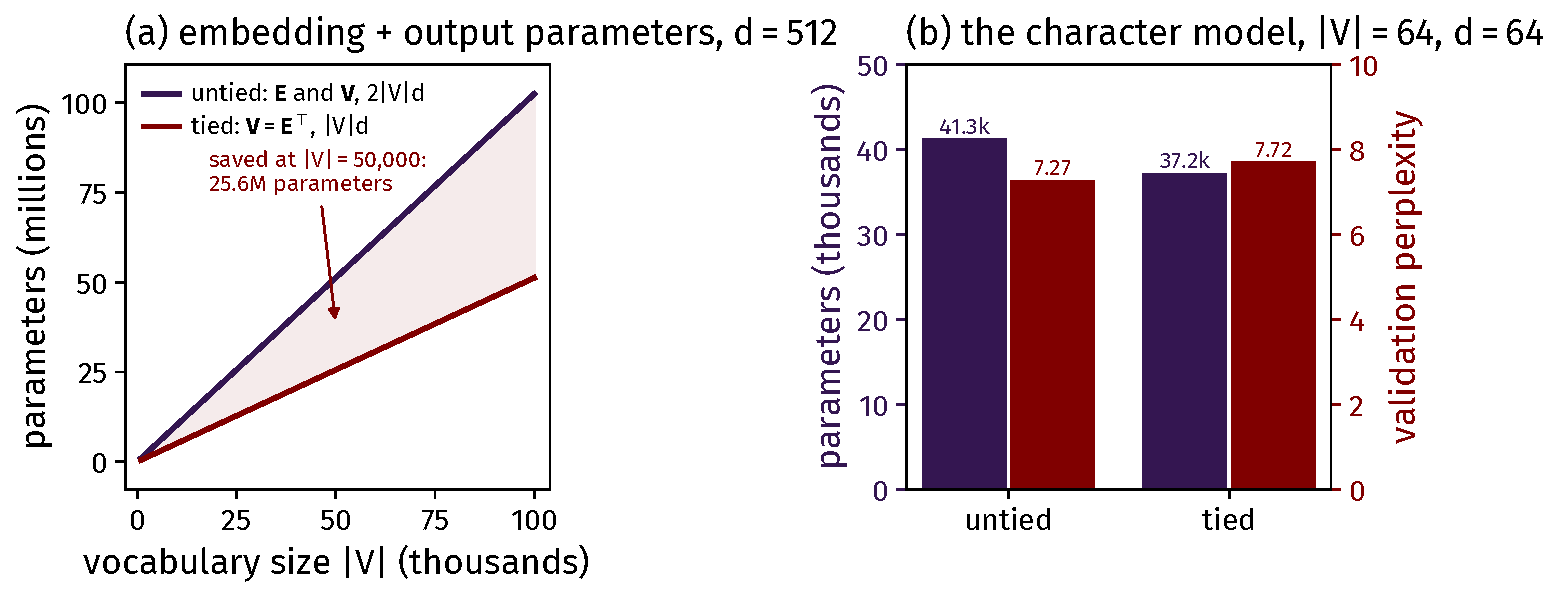
\includegraphics[width=0.82\linewidth]{weight_tying}
  \end{center}
  \vspace{-0.6em}
  {\tiny\color{mcMuted}
  (a) embedding and output parameters against vocabulary size at
  $d = 512$: tying halves them. (b) the character model trained here both
  ways: at $|V| = 64$ the saving is $4$k of $41$k parameters, and on this
  small text the untied model reaches a slightly lower validation
  perplexity ($7.27$ against $7.72$). The saving scales with $|V|$; the
  perplexity gain the book reports is for word vocabularies.
  \hfill Jurafsky \& Martin (2026), \S14.2.3.\par}
\end{frame}

% =====================================================================
\section{Labelling and Classification}
% =====================================================================

\begin{frame}{Sequence labelling: a label at every step}
  \vspace{-0.4em}
  \begin{center}
    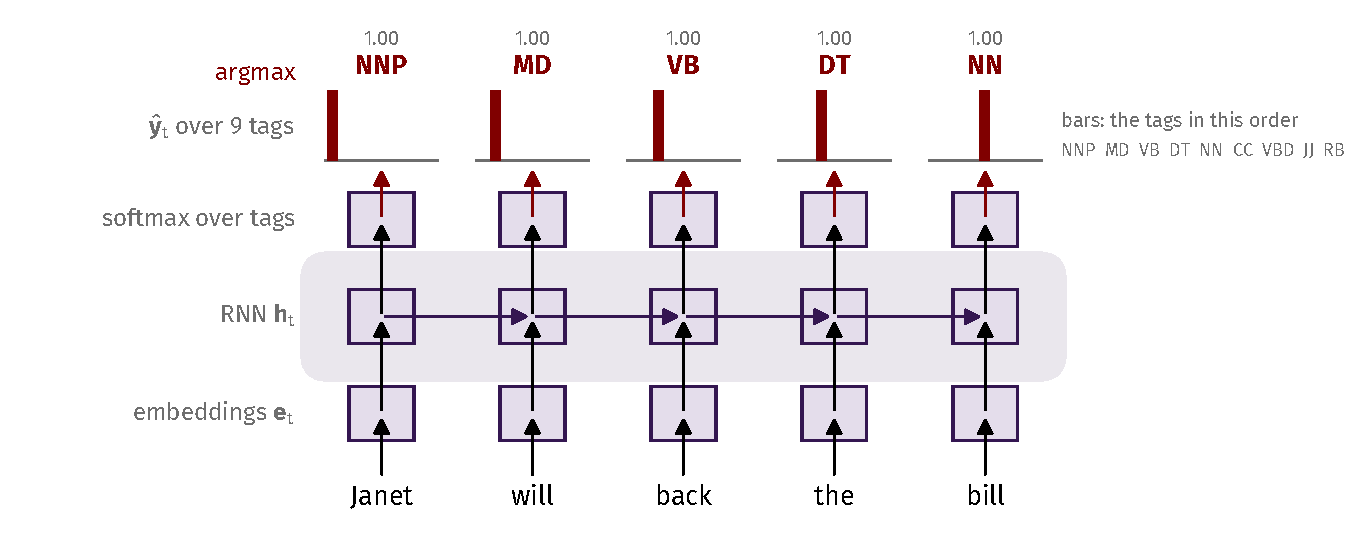
\includegraphics[width=0.80\linewidth]{pos_tagging}
  \end{center}
  \vspace{-0.6em}
  {\tiny\color{mcMuted}
  Part-of-speech tagging as sequence labelling: embeddings in, an RNN,
  and a softmax over the tag set at every step; the tag is the argmax ---
  the language model's output layer with the tag set in place of the
  vocabulary, the cross-entropy summed over the steps, and a local
  decision at each. The distributions shown are those of the
  left-to-right tagger trained here on a small grammar with $9$ tags,
  for the book's sentence.
  \hfill Layout of Jurafsky \& Martin (2026), Fig.~14.7; \S14.3.1.\par}
\end{frame}

\begin{frame}{Sequence classification: one label per sequence}
  \vspace{-0.55em}
  \begin{defx}[Read-outs for classification]\label{th:readout}
    \small
    Run the RNN over $x_1 \ldots x_n$ and pass one vector to a
    feedforward classifier with a softmax over the classes; three
    choices of the vector:
    \[
      \mathbf{h}_n \quad\text{(the last state)}, \qquad
      \mathbf{h}_{\mathrm{mean}} = \frac{1}{n}\sum_{i=1}^{n}\mathbf{h}_i, \qquad
      \mathbf{h}_{\mathrm{max}} = \max_{i}\,\mathbf{h}_i \ \text{(elementwise)}.
    \]
  \end{defx}
  \vspace{-0.1em}
  {\footnotesize
  \begin{itemize}\itemsep0.16em
    \item No loss at earlier positions: the one error signal goes
          back through the classifier, then the RNN --- \alert{end-to-end
          training}. $\mathbf{h}_n$ must carry the whole text; pooling
          reads every state
  \end{itemize}}
  \vspace{-0.3em}
  \srcline{Jurafsky \& Martin (2026), \S14.3.2, Eq.~14.15, Fig.~14.8.}
\end{frame}

\begin{frame}{Why the read-out matters}
  \vspace{-0.45em}
  \begin{propx}[Gradient paths of the three read-outs]\label{th:paths}
    \small
    Let $L$ be the classification loss. For the last-state read-out the
    gradient reaches $\mathbf{h}_t$ only through $n - t$ recurrent steps,
    $\partial L/\partial\mathbf{h}_t = (\partial L/\partial\mathbf{h}_n)\,
    \prod_{s=t+1}^{n}\mathbf{J}_s$; for the mean it also arrives directly,
    with weight $1/n$; for the max, with weight $1$ on every coordinate
    where $\mathbf{h}_t$ attains the max.
  \end{propx}
  \vspace{-0.1em}
  {\footnotesize
  \begin{itemize}\itemsep0.12em
    \item \focus{1}{Proof. Chain rule along the unrolled graph: the last
          state has one path back, the recurrence; the pooled read-outs
          add an edge from every $\mathbf{h}_t$ to the read-out, whose
          derivative is $\tfrac{1}{n}\mathbf{I}$ or a $0$/$1$ mask.
          \hfill $\square$}
    \item \focus{2}{By Class 28, the product $\prod \mathbf{J}_s$ shrinks
          geometrically for a simple cell; the direct edge does not. If
          the evidence is at the start of a long text, the last-state
          classifier may never see it during training.}
  \end{itemize}}
  \vspace{-0.3em}
  \srcline{Jurafsky \& Martin (2026), \S14.3.2, in words; Class 28, Proposition~2.}
\end{frame}

\begin{frame}{The three read-outs, measured}
  \begin{center}
    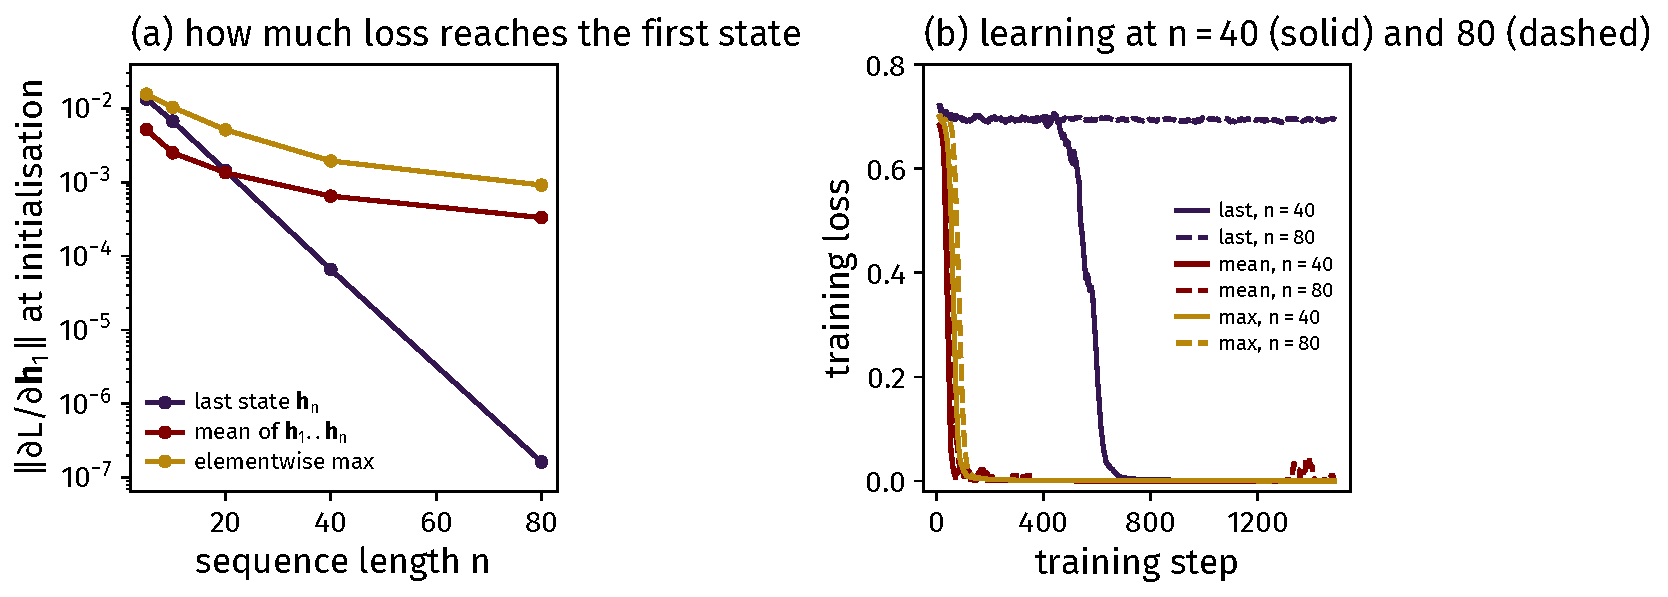
\includegraphics[width=0.88\linewidth]{pooling}
  \end{center}
  \vspace{-0.6em}
  {\tiny\color{mcMuted}
  A simple-RNN classifier ($d = 16$) on sequences whose label is decided
  by one marker among the first three symbols, the rest filler. (a) the
  gradient reaching $\mathbf{h}_1$ at initialisation, read off the tape:
  through the last state it falls by $10^{-5}$ from $n = 5$ to $80$; through
  the mean and the max it barely moves. (b) training at fixed length:
  at $n = 40$ the last-state model sits at chance for $500$ steps before
  it learns; at $n = 80$ it never does, while both pooled models
  learn within $100$ steps.
  \hfill Jurafsky \& Martin (2026), \S14.3.2.\par}
\end{frame}

% =====================================================================
\section{Stacking and Direction}
% =====================================================================

\begin{frame}{RNNs as modules}
  \vspace{-0.4em}
  \begin{center}
    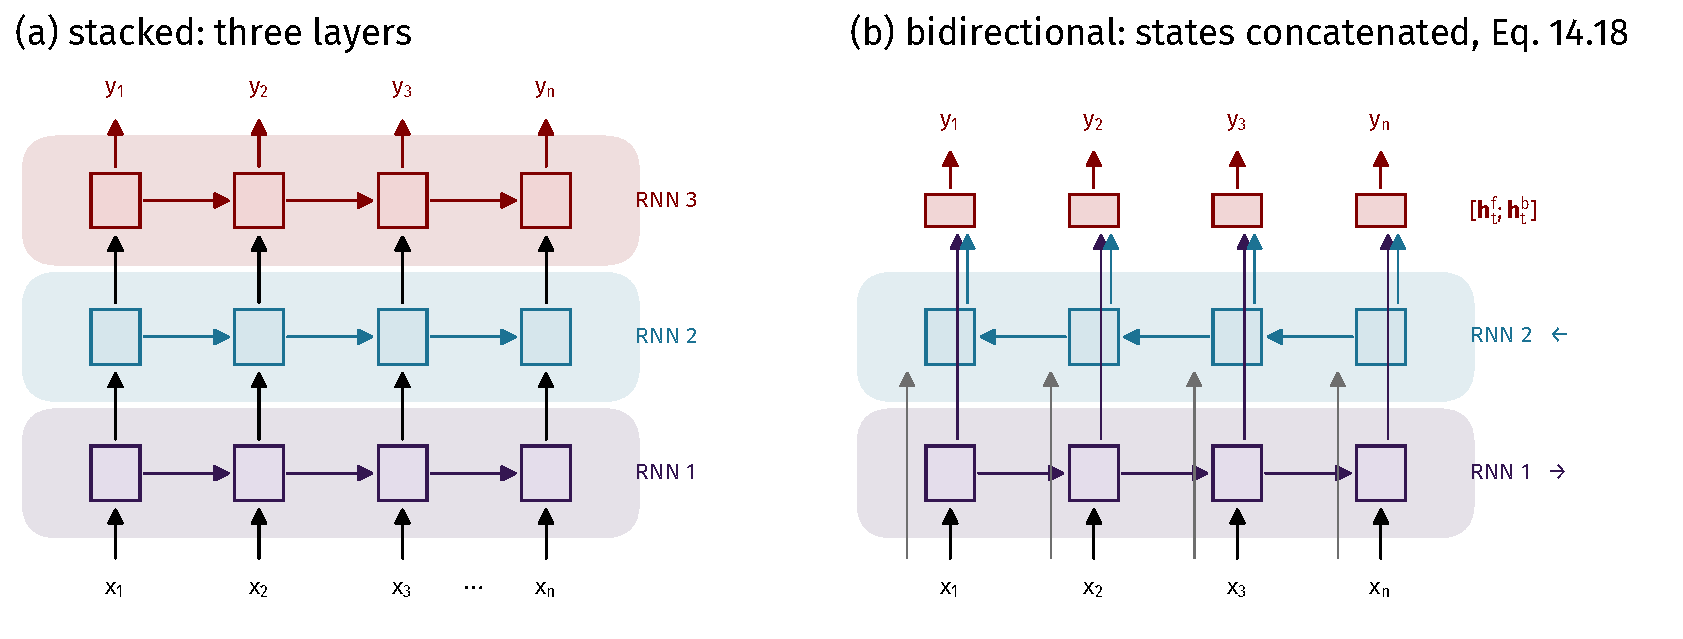
\includegraphics[width=0.84\linewidth]{stacked_bidirectional}
  \end{center}
  \vspace{-0.6em}
  {\tiny\color{mcMuted}
  Unrolled, an RNN is a feedforward graph with vectors in and out, so it
  composes like any other layer. (a) stacked: the output sequence of one
  layer is the input sequence of the next; the top layer's outputs are
  the final outputs. (b) bidirectional: one network reads left to right,
  one right to left, and their states at each step are concatenated.
  \hfill Layouts of Jurafsky \& Martin (2026), Figs.~14.10--14.11; \S14.4.\par}
\end{frame}

\begin{frame}{Stacking: depth per time step}
  \vspace{-0.45em}
  \begin{propx}[What stacking buys]\label{th:stack}
    \small
    $L$ layers of width $d$ cost $O(L d^2)$ recurrent parameters, the
    same as one layer of width $\sqrt{L}\,d$. At equal parameter count
    the stacked network is deeper between $\mathbf{x}_t$ and $\hat{\mathbf{y}}_t$
    ($L$ nonlinearities instead of one) and no deeper across time.
  \end{propx}
  \vspace{-0.1em}
  {\footnotesize
  \begin{itemize}\itemsep0.12em
    \item \focus{1}{Proof. Each layer has $\mathbf{U}, \mathbf{W} \in
          \mathbb{R}^{d \times d}$, so $2d^2$ per layer; one layer of width
          $d' = \sqrt{L}\,d$ has $2Ld^2$. The path from $\mathbf{h}^{(\ell)}_t$
          to $\mathbf{h}^{(\ell)}_{t+1}$ is still one step. \hfill $\square$}
    \item \focus{2}{Goodfellow's three ways to make an RNN deep: (a)
          stack the state hierarchically; (b) put an MLP in the
          input-to-hidden, hidden-to-hidden or hidden-to-output map ---
          which lengthens the shortest path across time; (c) add skip
          connections to shorten it again.}
    \item \focus{3}{Jurafsky: lower layers induce representations the
          upper layers use; the right depth is task-specific.}
  \end{itemize}}
  \vspace{-0.3em}
  \srcline{Jurafsky \& Martin (2026), \S14.4.1; Goodfellow et al.\ (2016), \S10.5, Fig.~10.13; Graves et al.\ (2013); Pascanu et al.\ (2014).}
\end{frame}

\begin{frame}{Stacking, tried at matched parameters}
  \begin{center}
    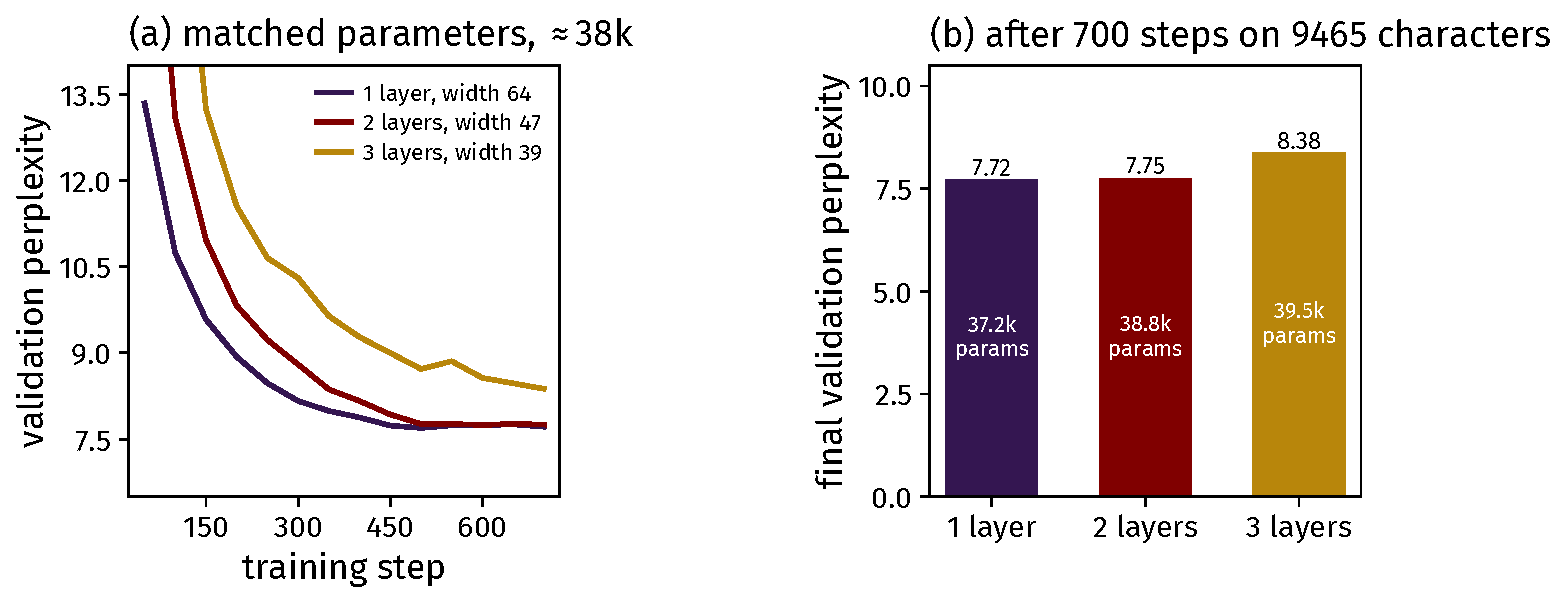
\includegraphics[width=0.88\linewidth]{stacked_depth}
  \end{center}
  \vspace{-0.6em}
  {\tiny\color{mcMuted}
  One, two and three LSTM layers, widths $64$, $47$, $39$, each about
  $38$k parameters, trained the same way on the character task. (a)
  validation perplexity by step; (b) at the end, $7.72$, $7.75$, $8.38$:
  on $9{,}465$ characters depth does not pay, and three layers are
  slower to train. The gain the books report is for data that has
  levels of abstraction to find.
  \hfill Jurafsky \& Martin (2026), \S14.4.1; Goodfellow et al.\ (2016), \S10.5.\par}
\end{frame}

\begin{frame}{Bidirectionality: the right context}
  \vspace{-0.45em}
  \begin{defx}[Bidirectional RNN, as used]\label{th:bi}
    \small
    Two independent RNNs, concatenated at each step:
    \[
      \mathbf{h}^{f}_t = \mathrm{RNN}_{\mathrm{forward}}(x_1, \ldots, x_t), \qquad
      \mathbf{h}^{b}_t = \mathrm{RNN}_{\mathrm{backward}}(x_t, \ldots, x_n), \qquad
      \mathbf{h}_t = [\mathbf{h}^{f}_t ; \mathbf{h}^{b}_t].
    \]
  \end{defx}
  \vspace{-0.1em}
  {\footnotesize
  \begin{itemize}\itemsep0.16em
    \item $\mathbf{h}^{f}_t$ is the ordinary state, everything to the left;
          $\mathbf{h}^{b}_t$ the state of a network run on the reversed
          input, everything to the right
    \item \alert{Labelling}: the decision at $t$ sees both sides.
          \alert{Classification}: concatenate the two final states, so the
          beginning counts as much as the end. Needs the whole input, so
          not for generation
  \end{itemize}}
  \vspace{-0.3em}
  \srcline{Jurafsky \& Martin (2026), \S14.4.2, Eqs.~14.16--14.18, Figs.~14.11--14.12; Schuster \& Paliwal (1997); Class 26.}
\end{frame}

\begin{frame}{Bidirectionality, measured}
  \begin{center}
    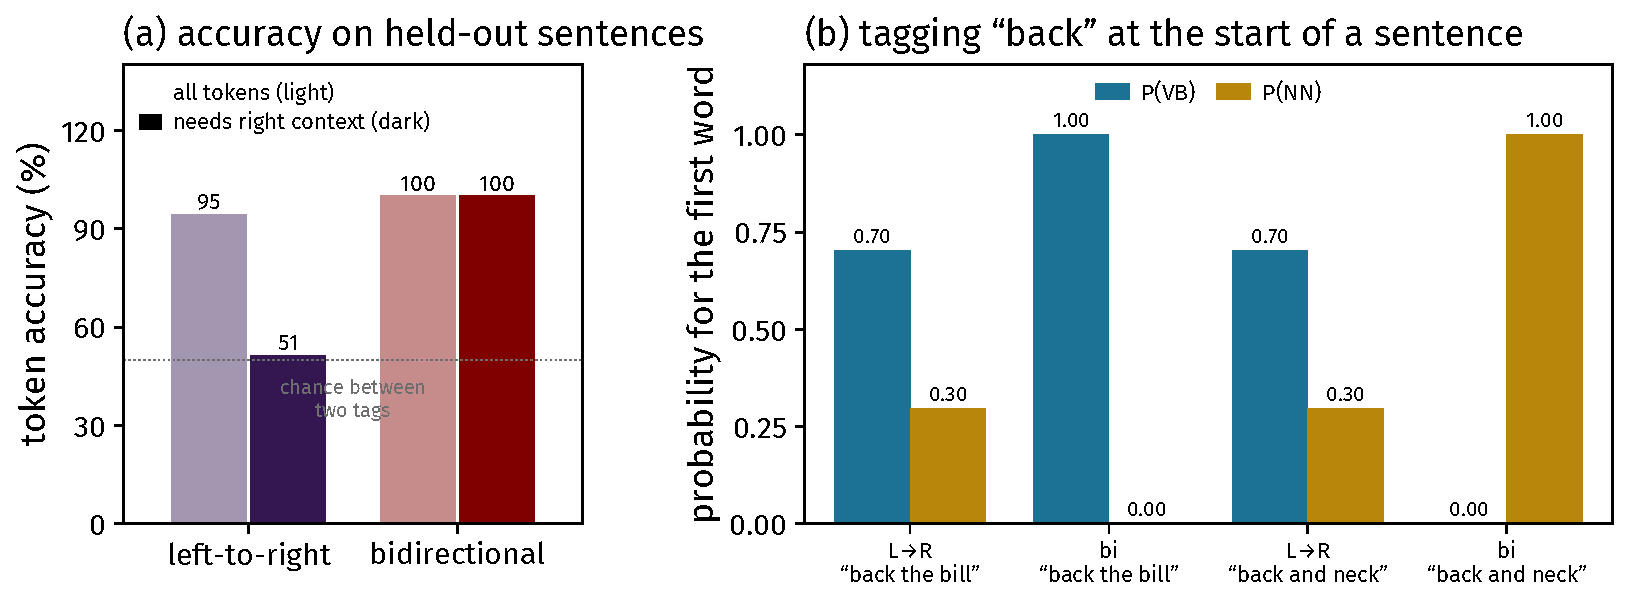
\includegraphics[width=0.90\linewidth]{bidirectional_labelling}
  \end{center}
  \vspace{-0.6em}
  {\tiny\color{mcMuted}
  Two taggers trained here on a grammar in which a word such as
  \emph{back} opens either an imperative (\emph{back the bill}: VB) or a
  noun phrase (\emph{back and neck ached}: NN). (a) on held-out
  sentences the left-to-right tagger scores $95\%$ overall but $51\%$ on
  those sentence-initial words --- chance between two tags, since at
  $t = 1$ it has seen nothing else; the bidirectional tagger scores $100\%$.
  (b) its distributions for \emph{back}: the same $0.7/0.3$ in both
  sentences for the left-to-right model, and the right answer for the
  bidirectional one.
  \hfill Jurafsky \& Martin (2026), \S14.4.2.\par}
\end{frame}

% =====================================================================
\section{The RNN as a Probabilistic Model}
% =====================================================================

\begin{frame}{The RNN as a directed graphical model}
  \vspace{-0.6em}
  \begin{propx}[Parameter sharing over the complete graph]\label{th:gm}
    \small
    An RNN over $y^{(1)} \ldots y^{(\tau)}$ with no other input defines
    $P(\mathbf{Y}) = \prod_{t=1}^{\tau} P\big(y^{(t)} \mid y^{(t-1)}, \ldots, y^{(1)}\big)$,
    with $L = \sum_t L^{(t)}$ and $L^{(t)} = -\log P\big(y^{(t)} \mid y^{(<t)}\big)$:
    the complete graph over the $y$'s. A tabular parametrisation with
    $k$-valued $y$ needs $O(k^{\tau})$ parameters; the RNN's count is $O(1)$ in $\tau$.
  \end{propx}
  \vspace{-0.1em}
  {\footnotesize
  \begin{itemize}\itemsep0.12em
    \item \focus{1}{Proof. The chain rule of probability gives the
          product; every conditional has the whole past as parents. The
          table for $P(y^{(\tau)} \mid y^{(<\tau)})$ alone has $k^{\tau}$
          entries; the RNN reuses $f$ and $\theta$ at every step.
          \hfill $\square$}
    \item \focus{2}{The state makes it possible: every stage has the same
          structure and parameters; a distant $y^{(i)}$ reaches $y^{(t)}$ through $h^{(t)}$.}
  \end{itemize}}
  \vspace{-0.3em}
  \srcline{Goodfellow et al.\ (2016), \S10.2.3, Eqs.~10.29--10.33.}
\end{frame}

\begin{frame}{The two graphs, drawn}
  \vspace{-0.3em}
  \begin{center}
  \begin{tikzpicture}[>=Stealth, font=\scriptsize, x=1.1cm, y=0.95cm,
      yn/.style={circle, draw=dpc, fill=dpc!8, line width=0.8pt, minimum size=0.5cm, inner sep=0pt},
      hn/.style={circle, draw=tealc, fill=tealc!8, line width=0.8pt, minimum size=0.5cm, inner sep=0pt},
      ar/.style={->, line width=0.7pt}]
    % complete graph
    \foreach \i in {1,...,5}{ \node[yn] (a\i) at (\i, 0) {$y^{(\i)}$}; }
    \foreach \i in {1,...,4}{ \pgfmathtruncatemacro{\j}{\i+1} \draw[ar, dpc] (a\i) -- (a\j); }
    \foreach \i/\j/\b in {1/3/45, 2/4/45, 3/5/45, 1/4/60, 2/5/60, 1/5/70}{
      \draw[ar, dpc!60] (a\i) to[bend left=\b] (a\j); }
    \node[mcMuted, anchor=west, font=\tiny] at (0.4, -0.75) {(a) the complete graph: every past $y^{(i)}$ is a parent of $y^{(t)}$};
    % with states
    \begin{scope}[xshift=7.2cm]
    \foreach \i in {1,...,5}{ \node[hn] (h\i) at (\i, 1.0) {$h^{(\i)}$}; \node[yn] (b\i) at (\i, 0) {$y^{(\i)}$}; }
    \foreach \i in {1,...,4}{ \pgfmathtruncatemacro{\j}{\i+1} \draw[ar, tealc] (h\i) -- (h\j); \draw[ar, dpc] (b\i) -- (h\j); }
    \foreach \i in {1,...,5}{ \draw[ar, tealc] (h\i) -- (b\i); }
    \node[mcMuted, anchor=west, font=\tiny] at (0.2, -0.75) {(b) with the state: the same structure and parameters at every stage};
    \end{scope}
  \end{tikzpicture}
  \end{center}
  \vspace{-0.2em}
  {\footnotesize
  \begin{itemize}\itemsep0.16em
    \item Marginalise the states out of (b) and (a) remains; keep them
          and $y^{(t)}$ reaches everything before through $h^{(t)}$
    \item The price: \alert{stationarity}, the same conditional at every
          $t$; and some operations stay hard, such as filling a gap in
          the middle
  \end{itemize}}
  \vspace{-0.3em}
  \srcline{Goodfellow et al.\ (2016), Figs.~10.7--10.8, \S10.2.3.}
\end{frame}

\begin{frame}{Deciding when to stop}
  \vspace{0.05em}
  {\footnotesize
  \begin{itemize}\itemsep0.3em
    \item A model over sequences must also decide their \alert{length}.
          Three mechanisms, all trained from data:
    \item \alert{An end symbol} $\langle/s\rangle$ in the vocabulary, inserted
          after the last token of every training sequence; sampling stops
          when it is drawn. This is Class 27's decoder and today's language
          model
    \item \alert{A Bernoulli output} at every step, a sigmoid trained by
          cross-entropy to say ``continue'' or ``halt''; works for any
          output type, real-valued sequences included
    \item \alert{Predict $\tau$ first}, then sample $\tau$ steps, feeding
          $\tau$ or $\tau - t$ back as an extra input so the model knows how
          close the end is:
          \[
            P(x^{(1)}, \ldots, x^{(\tau)}) = P(\tau)\,P(x^{(1)}, \ldots, x^{(\tau)} \mid \tau)
          \]
  \end{itemize}}
  \srcline{Goodfellow et al.\ (2016), \S10.2.3, Eq.~10.34; Schmidhuber (2012).}
\end{frame}

\begin{frame}{The tree-shaped cousin: recursive networks}
  \vspace{-0.3em}
  \begin{columns}[T, onlytextwidth]
    \begin{column}{0.44\textwidth}
      \begin{center}
      \begin{tikzpicture}[>=Stealth, font=\scriptsize, x=0.9cm, y=0.72cm,
          n/.style={circle, draw=shc, fill=shc!8, line width=0.8pt, minimum size=0.46cm, inner sep=0pt},
          xn/.style={circle, draw=tealc, fill=tealc!8, line width=0.8pt, minimum size=0.46cm, inner sep=0pt},
          on/.style={circle, draw=dpc, fill=dpc!8, line width=0.8pt, minimum size=0.46cm, inner sep=0pt},
          ar/.style={->, line width=0.7pt}]
        \foreach \i in {1,...,4}{ \node[xn] (x\i) at (\i, 0) {$x^{(\i)}$}; \node[n] (v\i) at (\i, 0.9) {}; \draw[ar, tealc] (x\i) -- (v\i); }
        \node[n] (l) at (1.5, 1.8) {}; \node[n] (r) at (3.5, 1.8) {}; \node[n] (t) at (2.5, 2.7) {};
        \draw[ar, shc] (v1) -- (l); \draw[ar, shc] (v2) -- (l); \draw[ar, shc] (v3) -- (r); \draw[ar, shc] (v4) -- (r);
        \draw[ar, shc] (l) -- (t); \draw[ar, shc] (r) -- (t);
        \node[on] (o) at (2.5, 3.6) {$o$}; \draw[ar, dpc] (t) -- (o);
        \node[dpc, anchor=west] at (3.0, 3.6) {$y$, $L$};
        \node[shc, anchor=west] at (1.85, 2.35) {$\mathbf{U}, \mathbf{W}$};
        \node[tealc, anchor=west] at (4.3, 0.45) {$\mathbf{V}$};
      \end{tikzpicture}
      \end{center}
      \vspace{-0.2em}
      {\tiny\color{mcMuted} A recursive network: a chain becomes a tree,
      with one set of weights at every node. \hfill Layout of Goodfellow et al.\ (2016), Fig.~10.14.\par}
    \end{column}
    \begin{column}{0.54\textwidth}
      \vspace{0.2em}
      {\footnotesize
      \begin{itemize}\itemsep0.24em
        \item The same idea as the RNN --- one function, one parameter
              set, applied repeatedly --- on a \alert{tree} instead of a
              chain; a variable-length sequence still maps to one vector
        \item Depth: the number of nonlinear compositions from a leaf to
              the root is $O(\log \tau)$ for a balanced tree, against
              $\tau$ for the chain, which helps with long dependencies
        \item The open question is the tree: fixed and balanced, given
              by a parser (the sentence's parse tree, Socher et al.), or
              inferred by the learner
      \end{itemize}}
    \end{column}
  \end{columns}
  \srcline{Goodfellow et al.\ (2016), \S10.6, Fig.~10.14; Pollack (1990); Socher et al.\ (2011, 2013).}
\end{frame}

% =====================================================================
\section{Putting It Together}
% =====================================================================

\begin{frame}{Four architectures}
  \vspace{-0.4em}
  \begin{center}
    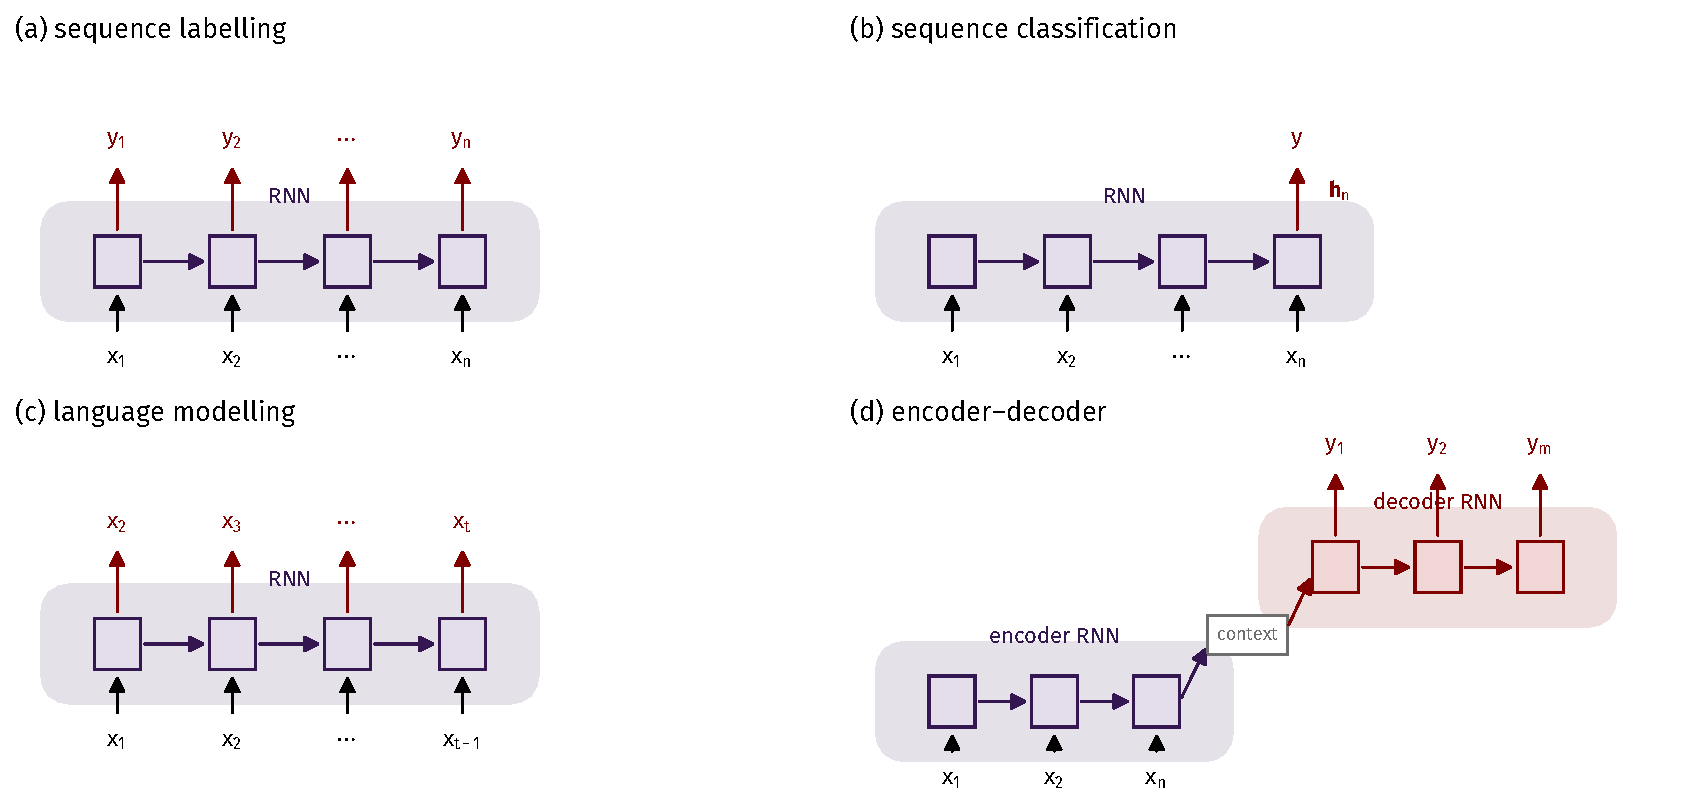
\includegraphics[width=0.82\linewidth]{four_architectures}
  \end{center}
  \vspace{-0.6em}
  {\tiny\color{mcMuted}
  (a) sequence labelling: each $x_i$ to a $y_i$. (b) classification: the
  whole sequence to one class, through the last state or a pooled one.
  (c) language modelling: the next token at every step. (d)
  encoder--decoder: one RNN maps the input to a context, another maps
  the context to an output sequence of its own length.
  \hfill Layout of Jurafsky \& Martin (2026), Fig.~14.15.\par}
\end{frame}

\begin{frame}{The block, in one table}
  \vspace{0.2em}
  {\scriptsize
  \renewcommand{\arraystretch}{1.36}
  \begin{tabular}{@{}l@{\hspace{1.0em}}l@{\hspace{1.0em}}l@{\hspace{1.0em}}l@{}}
    & \textbf{output} & \textbf{loss} & \textbf{where the gradient enters}\\
    language model & $\hat{\mathbf{y}}_t$ over $V$, every step & $-\log \hat{y}_t[w_{t+1}]$, averaged & every step\\
    sequence labelling & $\hat{\mathbf{y}}_t$ over tags, every step & cross-entropy, every step & every step\\
    classification & one softmax & one cross-entropy & $\mathbf{h}_n$, or every $\mathbf{h}_t$ if pooled\\
    encoder--decoder (27) & $\hat{\mathbf{y}}_t$ over $V$, decoder steps & teacher-forced cross-entropy & decoder steps, back through $\mathbf{c}$\\
    \multicolumn{4}{c}{}\\[-0.9em]
    stacked & top layer's outputs & as above & through $L$ cells per step\\
    bidirectional & $[\mathbf{h}^{f}_t ; \mathbf{h}^{b}_t]$ & as above & from both directions\\
  \end{tabular}}
  \vspace{0.6em}

  \begin{redhighlight}
    One cell, three matrices, and the choice of what to read out and
    where to pay the loss: that choice is the architecture.
  \end{redhighlight}
\end{frame}

\begin{frame}{Takeaways}
  \vspace{-0.1em}
  {\scriptsize
  \begin{enumerate}\itemsep0.24em
    \item A language model is an RNN whose output is the next token;
          it trains on raw text by self-supervision, and its loss is the
          log of its perplexity (Definition~\ref{th:lm},
          Proposition~\ref{th:ppl})
    \item Tying the output matrix to the embeddings removes $|V|\,d$
          parameters (Definition~\ref{th:tying}, Proposition~\ref{th:tyingcount});
          sampling with a temperature reads the model as a distribution
    \item Labelling emits a distribution at every step; classification
          reads out one vector, and pooling gives the early tokens a
          direct path to the loss (Definition~\ref{th:readout},
          Proposition~\ref{th:paths}) --- measured: at $n = 80$ the last-state
          classifier never learns, the pooled ones do
    \item Stacking buys depth per step at the same parameter count
          (Proposition~\ref{th:stack}); bidirectionality buys the right
          context (Definition~\ref{th:bi}) --- measured: $51\% \to 100\%$
          on the tokens that need it
    \item The RNN is the complete graphical model over the sequence
          with $O(1)$ parameters in its length (Proposition~\ref{th:gm});
          the recursive net is the same idea on a tree
  \end{enumerate}}
  \vspace{-0.2em}
  \bridge{Classes 30--31: the recurrence goes, attention stays --- the transformer.}
\end{frame}

\begin{frame}[allowframebreaks]{References}
  {\scriptsize
  \begin{itemize}\itemsep0.3em
    \item Jurafsky, D. \& Martin, J. H. (2026). \emph{Speech and Language
          Processing}, 3rd ed.\ draft, August 2026. Ch.~14, \S14.2--14.4,
          14.6; \S3.3, \S3.7; \S7.6.
    \item Goodfellow, I., Bengio, Y. \& Courville, A. (2016). \emph{Deep
          Learning}. MIT Press. \S10.2.3, \S10.3, \S10.5--10.6.
    \item Mikolov, T., Karafi\'at, M., Burget, L., \v{C}ernock\'y, J. \&
          Khudanpur, S. (2010). Recurrent neural network based language
          model. \emph{Interspeech}.
    \item Elman, J. L. (1990). Finding structure in time. \emph{Cognitive
          Science}, 14, 179--211.
    \item Press, O. \& Wolf, L. (2017). Using the output embedding to
          improve language models. \emph{EACL}.
    \item Inan, H., Khosravi, K. \& Socher, R. (2017). Tying word vectors
          and word classifiers. \emph{ICLR}.
    \item Schuster, M. \& Paliwal, K. K. (1997). Bidirectional recurrent
          neural networks. \emph{IEEE Trans.\ Signal Processing}, 45,
          2673--2681.
    \item Graves, A., Mohamed, A. \& Hinton, G. (2013). Speech recognition
          with deep recurrent neural networks. \emph{ICASSP}.
    \item Pascanu, R., Gulcehre, C., Cho, K. \& Bengio, Y. (2014). How to
          construct deep recurrent neural networks. \emph{ICLR}.
    \item Graves, A. (2013). Generating sequences with recurrent neural
          networks. arXiv:1308.0850.
    \item Shannon, C. E. (1951). Prediction and entropy of printed
          English. \emph{Bell System Technical Journal}, 30, 50--64.
    \item Schmidhuber, J. (2012). Self-delimiting neural networks.
          arXiv:1210.0118.
    \item Pollack, J. B. (1990). Recursive distributed representations.
          \emph{Artificial Intelligence}, 46, 77--105.
    \item Socher, R., Lin, C. C., Ng, A. Y. \& Manning, C. D. (2011).
          Parsing natural scenes and natural language with recursive
          neural networks. \emph{ICML}.
    \item Socher, R. et al.\ (2013). Recursive deep models for semantic
          compositionality over a sentiment treebank. \emph{EMNLP}.
    \item Henry, O. (1905). The Gift of the Magi. Public domain; the text
          the language model is trained on.
  \end{itemize}}
\end{frame}

\begin{frame}[standout]
  Questions?
\end{frame}

\end{document}
